\documentclass[conference,11pt]{IEEEtran}
\IEEEoverridecommandlockouts
% The preceding line is only needed to identify funding in the first footnote. If that is unneeded, please comment it out.
\usepackage{cite}
\usepackage{amsmath,amssymb,amsfonts}
\usepackage{algorithmic}
\usepackage{adjustbox}
\usepackage{graphicx}
\usepackage{textcomp}
\usepackage{xcolor}
\usepackage{listings}
\usepackage{mathtools}
\usepackage{qtree}
\usepackage{cancel}
\usepackage{enumitem}
\usepackage{float}
\usepackage{tikz}
\usepackage{mathtools}
\usepackage{semantic}
\usepackage{stmaryrd}
\usepackage{twoopt}
\usepackage{pgfplots}
\usepackage{bm}
\usepackage{IEEEtrantools}
\usepackage{cleveref}

\usetikzlibrary{automata, positioning, arrows, calc, shapes.multipart}
\DeclarePairedDelimiter{\ceil}{\lceil}{\rceil}
\DeclarePairedDelimiter{\floor}{\lfloor}{\rfloor}
\newcommand{\code}[1]{\mbox{\texttt{#1}}}
\newcommand{\unitvec}[1]{\boldsymbol{\widehat{#1}}}
\newcommand{\paren}[1]{\left( #1 \right)}
\newcommand{\brac}[1]{\left[ #1 \right]}
\newcommand{\cbrac}[1]{\left\{ #1 \right\}}
\newcommand{\dbrac}[1]{\left\llbracket #1 \right\rrbracket}
\newcommand{\deriv}[2]{\frac{d #1}{d #2}}
\newcommand{\nderiv}[3]{\frac{d^{#3} #1}{d #2^{#3}}}
\newcommand{\pderiv}[2]{\frac{\partial #1}{\partial #2}}
\newcommand{\npderiv}[3]{\frac{\partial^{#3} #1}{\partial #2^{#3}}}
\newcommand{\vo}{\vec{o}\@ifnextchar{^}{\,}{}}
\newcommand{\underbrack}[2]{\underbrace{#1}_{\substack{#2}}}
\newcommand{\REALS}{\mathbb{R}}
\newcommand{\NATURALS}{\mathbb{N}}
\newcommand{\INTEGERS}{\mathbb{Z}}
\renewcommand{\thesubsection}{\thesection.\alph{subsection}}
\newcommand{\cov}{\code{COV}}
\DeclarePairedDelimiter\abs{\lvert}{\rvert}
\DeclarePairedDelimiter\norm{\lVert}{\rVert}
\newcommand\exinf{\mathrel{\overset{\infty}{\exists}}}
\newcommand\fainf{\mathrel{\overset{\infty}{\forall}}}
\newcommand{\setcomp}[2]{\cbrac{#1\, \middle|\, #2}}
\newcommand{\powerset}[1]{2^{#1}}
\newcommand{\finitewords}{A_1A_2\ldots A_N \in \paren{\powerset{AP}}^+}
\newcommand{\infinitewords}{A_1A_2\ldots \in \paren{\powerset{AP}}^{\omega}}
\newcommand{\ltlalways}{\square}
\newcommand{\ltlnext}{\bigcirc}
\newcommand{\ltleventually}{\Diamond}
\newcommand{\ltland}{\wedge}
\newcommand{\ltlor}{\vee}
\newcommand{\ltluntil}{\mathbin{\bold{U}}}
\newcommand{\impl}{\rightarrow}
\newcommand{\nor}{\bar{\vee}}
\newcommand{\true}{\textbf{true}}
\newcommand{\false}{\textbf{false}}
\newcommand{\vocab}{\mathcal{V}}
\newcommand{\model}{\mathcal{M}}
\newcommand{\domain}{\mathcal{D}}
\newcommand{\interp}{\mathcal{I}}
\newcommand{\hoare}[3]{\cbrac{#1}\texttt{#2}\cbrac{#3}}
\DeclareMathOperator{\sign}{sign}
\DeclareMathOperator{\freevars}{freevars}
\DeclareMathOperator{\prim}{prime}
\DeclareMathOperator{\odd}{odd}
\DeclareMathOperator{\post}{post}
\newcommandtwoopt{\evalu}[3][\mathcal{M}][\rho]{\llbracket #3\rrbracket_{#1,#2}}
\tikzset{
  node distance=2cm, % specifies the minimum distance between two nodes. Change if necessary.
  initial text=$ $, % sets the text that appears on the start arrow
  accepting/.style={rectangle},
  state/.append style={circle},
  every edge/.style={draw,
    ->,>=stealth', % Makes edges directed with bold arrowheads
    auto,
    semithick},
  cfgedge/.style={rectangle, rounded corners, fill=gray!50, anchor=center}
}

\def\BibTeX{{\rm B\kern-.05em{\sc i\kern-.025em b}\kern-.08em
    T\kern-.1667em\lower.7ex\hbox{E}\kern-.125emX}}
\begin{document}

\title{Time and Energy Optimal Control for a Single Track Modeled Vehicle.}

\author{\IEEEauthorblockN{Anton Pozharskiy}
\IEEEauthorblockA{\textit{Albert-Ludwigs-Universität Freiburg}}
Freiburg, Germany \\
anton@pozhar.ski
\and
\IEEEauthorblockN{Mario Willaredt}
\IEEEauthorblockA{\textit{Albert-Ludwigs-Universität Freiburg}}
Freiburg, Germany \\
mario-willaredt@web.de
\and
\IEEEauthorblockN{Adil Younas}
\IEEEauthorblockA{\textit{Albert-Ludwigs-Universität Freiburg}}
Freiburg, Germany \\
adil.younas@gmx.de
}

\maketitle

\begin{abstract}
  This project sets out to formulate a true time optimal path finding problem for a rear wheel drive vehicle. The vehicle is modeled with linear in angle tire model, with slip limited via constraints.
  Progress is made towards use of a more complex nonlinear model that can, in conjunction with an efficient NLP solver (ACADOS \cite{Verschueren2021}), be used for optimal control of a race vehicle,
  and vehicle parameter optimization.
\end{abstract}

\begin{IEEEkeywords}
Optimal Control, Model Predictive Control, Tire Models, Time Optimal Control.
\end{IEEEkeywords}

\section{Introduction}
Optimal control has become a popular paradigm of controller design in a multitude of autonomous vehicle projects. There also exists prior work on model predictive control as applied specifically
to the target of the project: time optimal planning and control \cite{Verschueren2014a}\cite{LOT20147559}. In this project we attempt to formulate true time optimal controller that takes into
account a tire model with slip angles and independent tire forces. Generally optimal control and MPC algorithms must trade-off the complexity of the dynamic model and speed of the solver. In the
past work it is very common for the authors to use simple slip free bicycle model to implement the vehicle dynamics, however there are often interesting behaviors such as counter-steer and tire
dynamics that are not modeled.

The path planning aspect of the time optimal driving problem provides the primary difficulty of the approach taken in this project, along with the severe non-linearity introduced not just by the
tire model, but also by the commonly used time optimality reformulation that takes the ``speed of time'' as as an optimization variable. This non-linearity often leads to local minima and makes the
problem highly sensitive to initialization and hyper-parameters.

\section{Formulation}
\begin{figure}[t]
  \centering
  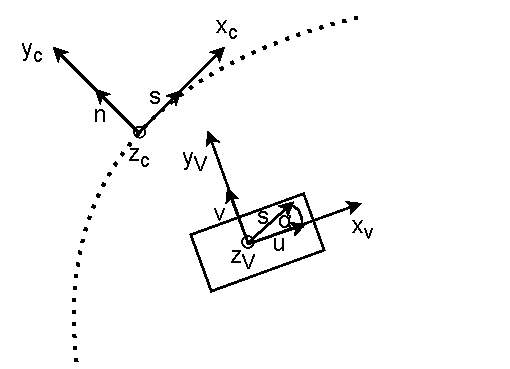
\includegraphics{curvilinear2.pdf}
  \caption{curvilinear coordinate system}
  \label{fig:curv}
\end{figure}
\subsection{Dynamics}
The model of the dynamic system can be broken up into the road model, the dynamics of the vehicle in the CG (center of gravity) frame, and the dynamics of the vehicle in the
curvilinear coordinate system.

\subsubsection{Road Model}
The first challenge in formulating a vehicle model is modeling the road surface, which is generally a long narrow strip. This combined with the fact that roads generally do not
form convex sets in euclidean space means that a different coordinate system is needed. For this purpose a curvilinear coordinate system is used. In this model the vehicle's
position is represented by the distance along the center-line of the road ($s$), the distance perpendicular to the center-line ($n$), and the relative angle $\alpha$ to the direction
of the road. The road's position in euclidean space is defined as in \cite{LOT20147559}, i.e. a normalized parametric curve which is defined by a single function $\kappa(s)$ which defines
the rate of change which gives us the road road center-line coordinates as:

\begin{IEEEeqnarray}{C}
  \IEEEyesnumber \IEEEyessubnumber*
  x' = cos(\theta) \label{eq:road1}\\
  y' = cos(\theta) \label{eq:road2}\\
  \theta' = \kappa(s) \label{eq:road3}
\end{IEEEeqnarray}

The $(s,n,\alpha)$ coordinate system is right handed as shown in Figure. \ref{fig:curv}. With this formulation the road is fully defined with the addition of a formalism for the road edges.
The problem formulation addressed by ACADOS limits us to a single width function $w(s)$, which defines the symmetric edges of the road $w_r$, $w_l$:
\begin{IEEEeqnarray}{C}
  \IEEEyesnumber \IEEEyessubnumber*
  w_r = -w(s) \label{eq:width1}\\
  w_l = w(s) \label{eq:width2}
\end{IEEEeqnarray}

\subsubsection{CG Dynamics}
The CG dynamics of the vehicle is modeled using a bicycle model (Figure. \ref{fig:cg}) that takes into account the slip angles and forces exerted by the front and rear tires independently.

The state space of the CG dynamics is as follows:
\begin{equation}
  x_{\mathrm{cg}} = 
  \begin{bmatrix}
    u\\
    v\\
    \omega\\
    \delta
  \end{bmatrix}
  \label{eq:state}
\end{equation}
The model has three degrees of freedom that are used as control variables: the brake torque $\tau_{b}$, the brake torque $\tau_{e}$, and the steering rate
$\omega_{\mathrm{steer}}$:
\begin{equation}
  \label{eq:control}
  u =
  \begin{bmatrix}
    \tau_{b}\\
    \tau_{e}\\
    \omega_{\mathrm{steer}}
  \end{bmatrix}
\end{equation}
The vehicle is modeled as rear wheel drive only.
\begin{figure}[b]
  \centering
  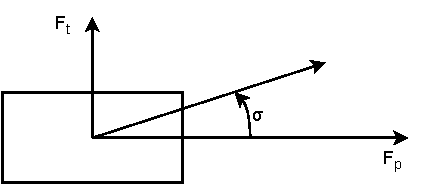
\includegraphics[scale=0.6]{tire_model.pdf}
  \caption{Forces acting on a tire.}
  \label{fig:tire}
\end{figure}
Each tire experiences two forces transverse and parallel to the rolling axis of the tire as shown in \Cref{fig:tire}. The parallel forces are defined as follows:

\begin{IEEEeqnarray}{C}
  \IEEEyesnumber \IEEEyessubnumber*
  F_{fp} = -k_{\mathrm{b}}\tau_{\mathrm{b}}(1-b_b) \label{eq:Ffp}\\
  F_{rp} = k_{\mathrm{e}}\tau_{\mathrm{e}}-k_{\mathrm{b}}\tau_{\mathrm{b}}b_b\label{eq:Frp}
\end{IEEEeqnarray}

The transverse forces are modeled as a linear w.r.t the slip angle of the tire. The direction of travel angles are defined as follows:

\begin{IEEEeqnarray}{C}
  \IEEEyesnumber \IEEEyessubnumber*
  \tan\gamma_r = \frac{v - l_r\omega}{u}\label{eq:dotr}\\
  \tan\gamma_f = \frac{v + l_f\omega}{u}\label{eq:dotf}
\end{IEEEeqnarray}

and the slip angles are:

\begin{IEEEeqnarray}{C}
  \IEEEyesnumber \IEEEyessubnumber*
  \sigma_r = \gamma_r \label{eq:slipr}\\
  \sigma_f = \gamma_f - \delta\label{eq:slipf}
\end{IEEEeqnarray}
the forces are then linear w.r.t the slip angles:
\begin{IEEEeqnarray}{C}
  \IEEEyesnumber \IEEEyessubnumber*
  F_{ft} = -K_f\sigma_f N_f \label{eq:Fft}\\
  F_{rt} = -K_r\sigma_r N_r\label{eq:Frt}
\end{IEEEeqnarray}

with $N_f$ and $N_r$ being the normal force on the tire in the front and rear respectively and are exactly:
\begin{IEEEeqnarray}{C}
  \IEEEyesnumber \IEEEyessubnumber*
  N_f = mg(1-m_b) \label{eq:Nf}\\
  N_r = mg(m_b)\label{eq:Nr}
\end{IEEEeqnarray}

The dynamics in the CG frame is then simply defined through simple euclidean kinematics with additional square terms for aerodynamic drag:

\begin{equation}
  \label{eq:cgdyn}
  \dot{x}_{\mathrm{cg}} =
  \begin{bmatrix}
    F_{rp} + F_{fp}\cos\delta - F_{ft}\sin\delta - C_uu^2\\
    F_{rf} + F_{fp}\sin\delta + F_{ft}\cos\delta - C_vv^2\\
    -l_rF_{rt} + l_f\paren{F_{ft}\cos\delta + F_{fp}\sin\delta}\\
    \omega_{\mathrm{steer}}
  \end{bmatrix}
\end{equation}

\begin{figure}[t]
  \centering
  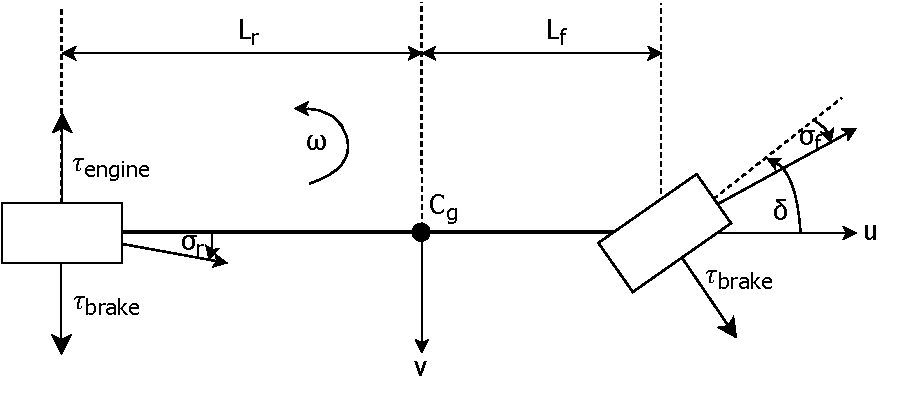
\includegraphics[scale=0.6]{vehicle_model.pdf}
  \caption{CG coordinate system}
  \label{fig:cg}
\end{figure}
\subsubsection{Vehicle Dynamics}
The dynamics of the vehicle in the curvilinear frame can be entirely separated from the CG dynamics as long as the CG dynamics provide $u$, $v$, and $\omega$.
The state of the system in the curvilinear state is:
\begin{equation}
  \label{eq:curvstate}
  x_{\mathrm{curv}}=
  \begin{bmatrix}
    s\\
    n\\
    \alpha
  \end{bmatrix}
\end{equation}
Given these states we can define the dynamics:

\begin{equation}
  \label{eq:curvdyn}
  \dot{x}_{\mathrm{curv}}=
  \begin{bmatrix}
    \frac{u\cos\alpha - v\sin\alpha}{1-n\kappa(s)}\\
    u\sin\alpha + v\cos\alpha\\
    \omega - \kappa(s)\frac{u\cos\alpha - v\sin\alpha}{1-n\kappa(s)}
  \end{bmatrix}
\end{equation}

With these dynamics defined the dynamics of the whole system are defined as:

\begin{IEEEeqnarray}{C}
  \IEEEyesnumber \IEEEyessubnumber*
  x_{\mathrm{dyn}} =
  \begin{bmatrix}
    x_{\mathrm{curv}}\\
    x_{\mathrm{cg}}
  \end{bmatrix}
  \label{eq:fullstate}\\
  \dot{x}_{\mathrm{dyn}} =
  \begin{bmatrix}
    \dot{x}_{\mathrm{curv}}\\
    \dot{x}_{\mathrm{cg}}
  \end{bmatrix}
  \label{eq:fulldyn}
\end{IEEEeqnarray}

\subsection{Problem Formulation}
\begin{figure}[t]
  \centering
  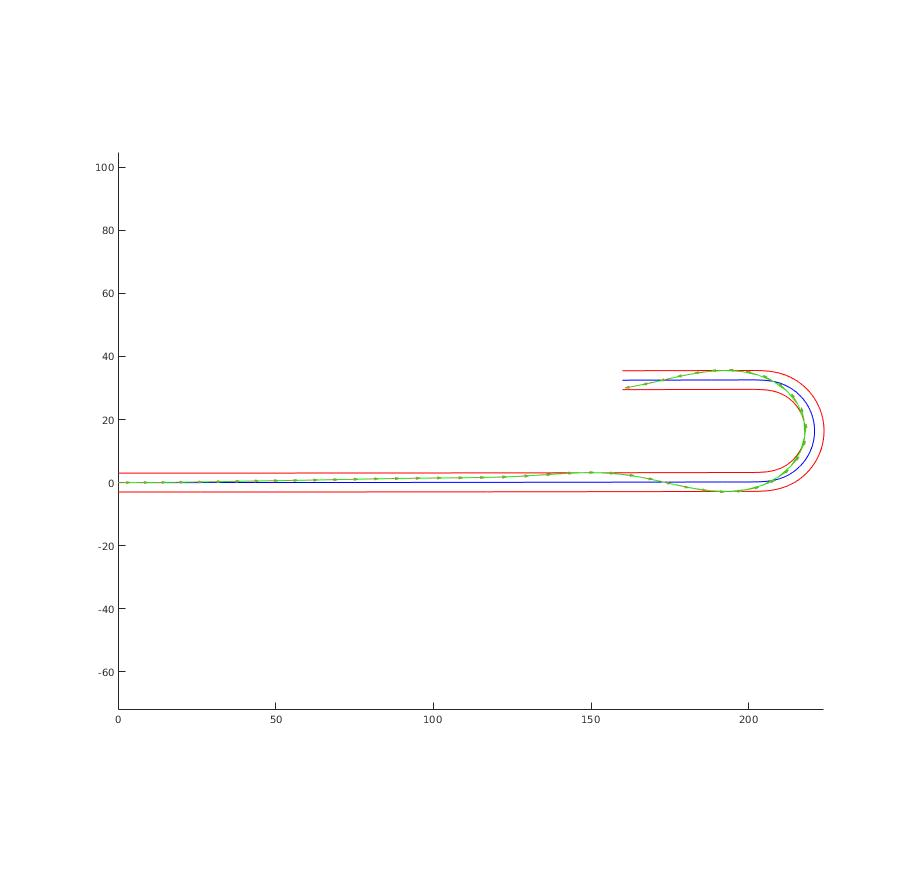
\includegraphics[scale=0.25]{hairpin_brake.jpg}
  \caption{Trajectory followed by the vehicle in the high speed hairpin experiment.}
  \label{fig:hptraj}
\end{figure}
\begin{figure}[b]
  \centering
  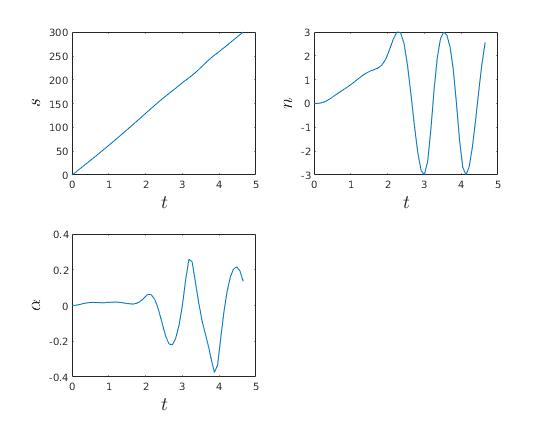
\includegraphics[scale=0.5]{hairpin_brake_curv.jpg}
  \caption{Curvilinear coordinates of vehicle in the high speed hairpin experiment.}
  \label{fig:hpcurv0}
\end{figure}
The MPC problem is solved using the ACADOS tool \cite{Verschueren2021}, which treats a specific problem formulation.
In order to formulate the time optimal problem, a new state $\Delta_t$ is introduced that represents the speed of time. This gives the normalized dynamics:
\begin{IEEEeqnarray}{C}
  \IEEEyesnumber \IEEEyessubnumber*
  x_{\mathrm{topt}} =
  \begin{bmatrix}
    x_{\mathrm{curv}}\\
    \Delta_t\\
    x_{\mathrm{cg}}
  \end{bmatrix}
  \label{eq:toptstate}\\
  \dot{x}_{\mathrm{topt}} = \Delta_t
  \begin{bmatrix}
    \dot{x}_{\mathrm{curv}}\\
    0\\
    \dot{x}_{\mathrm{cg}}
  \end{bmatrix}
  \label{eq:toptdyn}
\end{IEEEeqnarray}
These dynamics are reformulated into implicit dynamics in order to use the implicit Runge-Kutta methods provided in ACADOS:
\begin{equation}
  \label{eq:fimpl}
  f_{\mathrm{impl}}(x_{\mathrm{topt}},\dot{x}_{\mathrm{topt}},u)=
  \dot{x}_{\mathrm{topt}} - \Delta_t
  \begin{bmatrix}
    \dot{x}_{\mathrm{curv}}\\
    0\\
    \dot{x}_{\mathrm{cg}}
  \end{bmatrix}
\end{equation}
This then gives us the following formulation of the optimal control problem:
% TODO: figure out the correct way to do the alignment here.
\begin{IEEEeqnarray}{ll}
  \IEEEnonumber \displaystyle
  \min_{x_{\mathrm{topt}}(\cdot),u(\cdot)}\int_{0}^{1} \Delta_t^2&+10^{-6}\tau_{e}\tau_{b}\\
  \IEEEnonumber&+10^{-6}\tau_{e}^2\\
  \IEEEnonumber&+10^{-6}\tau_{b}^2\\ 
  \IEEEyesnumber\IEEEyessubnumber*&+10^{-6}\omega_{\mathrm{steer}}^2   \label{eq:prob1}
\end{IEEEeqnarray}

subject to the equality constraints with $\tau$ dependence dropped where convenient:

\begin{IEEEeqnarray}{rcl'r}
  \IEEEyessubnumber*
  f_{\mathrm{impl}}(x_{\mathrm{topt}},\dot{x}_{\mathrm{topt}},u) &=& 0 & \tau \in  (0,1]\label{eq:prob2}\\
  x_{\mathrm{curv}}(0) &=& x_{\mathrm{curv}0} &\label{eq:prob3}\\
  x_{\mathrm{cg}}(0) &=& x_{\mathrm{cg}0} &\label{eq:prob4}\\
  s(1) &=& s_{\mathrm{max}} &\label{eq:prob5}
\end{IEEEeqnarray}

And the inequality constraints:
\begin{IEEEeqnarray}{rcl'r}
  \IEEEyessubnumber*
  0&\le \Delta_t(0) \le& 3 &\label{eq:prob6}\\
  -1 &\le \frac{n(\tau)}{w(s(\tau))} \le& 1 & \tau \in  (0,1)\label{eq:prob7}\\
  -\frac{\pi}{2} &\le \alpha(\tau) \le& \frac{\pi}{2} & \tau \in  (0,1)\label{eq:prob8}\\
  -\frac{\pi}{4} &\le \delta(\tau) \le& \frac{\pi}{4} & \tau \in  (0,1)\label{eq:prob9}\\
  0 &\le \tau_e(\tau) \le& 1  & \tau \in  (0,1)\label{eq:prob10}\\
  0 &\le \tau_b(\tau) \le& 1 & \tau \in  (0,1)\label{eq:prob11}\\
  -0.5 &\le \omega_{\mathrm{steer}}(\tau) \le& 0.5 & \tau \in  (0,1)\label{eq:prob12}\\
  &F_{rp}^2 + F_{rt}^2 \le& (\mu N_r)^2 & \tau \in  (0,1)\label{eq:prob13}\\
  &F_{fp}^2 + F_{ft}^2 \le& (\mu N_f)^2 & \tau \in  (0,1)\label{eq:prob14}
\end{IEEEeqnarray}

The primary cost in Equation. (\ref{eq:prob1}) is the square of the speed of time variable $\Delta_t$. This enforces the time optimality target of the optimal control problem.
The cross term $\tau_e\tau_b$ is introduced to minimize application of engine torque and brakes at the same time, and the remaining cost terms are to enforce minimality of control inputs.
Equation (\ref{eq:prob2}) is the dynamics of the system, Equations (\ref{eq:prob3}), (\ref{eq:prob4}), and (\ref{eq:prob6}) set the initial conditions of the system including range of values that
the free variable of $\Delta_t$ can take. The remaining inequalities represent the physical limits of the system. In particular the last two inequalities are crucial to realistic modeling of the
vehicle and provide the grip limits of the tires, similarly to the approach taken in \cite{LOT20147559}.

In order to improve the convergence properties we introduce slack variables
with $L_1$ penalties to the inequalities in Equations (\ref{eq:prob7}), (\ref{eq:prob13}), and (\ref{eq:prob14}).


\section{Numerical Solution}
\begin{figure}[t]
  \centering
  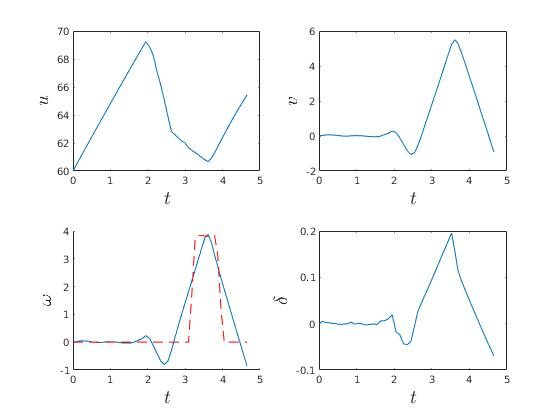
\includegraphics[scale=0.5]{hairpin_brake_cg.jpg}
  \caption{Center of gravity dynamics of the vehicle in the high speed hairpin experiment.}
  \label{fig:hpcg0}
\end{figure}
\begin{figure}[b]
  \centering
  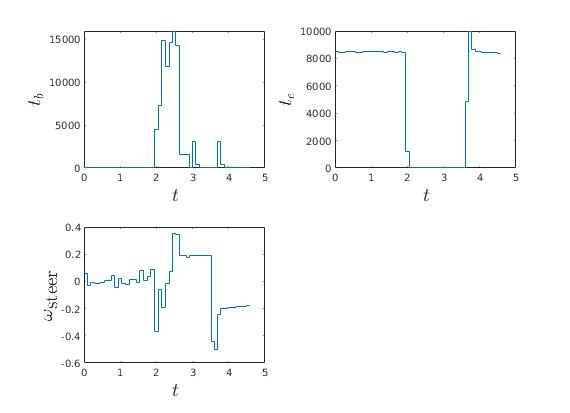
\includegraphics[scale=0.5]{hairpin_brake_u.jpg}
  \caption{Controls in the high speed hairpin experiment.}
  \label{fig:hpu0}
\end{figure}
\subsection{Solver Options}
The problem formulated above is solved using the ACADOS package. Due to inconsistency in convergence behavior from problem instance to problem instance some parameters were tuned specifically to
get convergent results. These will be discussed in the conclusions and further explorations sections of this report. However there were several consistent parameters that were used for
all the following experiments.

The dynamics are discretized using a 4th order implicit Runge-Kutta method with $N = 50$. Globalization is done through the merit function backtracking feature provided in the ACADOS package, using
default settings. The required stopping tolerances for stationarity and inequality are set to $10^{-4}$ and $10^{-5}$ respectively. The problem is then solved using the standard SQP (sequential
quadratic programming) approach (the real time iteration approach will be discussed in the Conclusions section). The QPs formed in the SQP method are solved using the partial condensing HPIPM
\cite{FRISON2003} method.
\begin{table}[t]
  \centering
  \begin{tabular}{l|r}
    Constant & Value \\\hline
    $m$& 1440 kg\\
    $I$&1730 kgm$^2$\\
    $l_f$&1.482 m\\
    $l_r$&1.118 m\\
    $k_e$&$10^4$\\
    $k_b$&$2\times 10^4$\\
    $b_b$&0.5\\
    $m_b$&0.5\\
    $K_r$&29\\
    $K_f$&29\\
    $C_u$&0.039$\frac{\mathrm{N}\mathrm{s}^2}{\mathrm{m}^2}$\\
    $C_v$&0.039$\frac{\mathrm{N}\mathrm{s}^2}{\mathrm{m}^2}$\\
    $\mu$&1.2\\
  \end{tabular}
  \caption{Vehicle constants}
  \label{tab:veh}
\end{table}
\subsection{Initialization and Warm Starting}
Initialization of the ACADOS solver plays a very important role in the convergence behavior of the controller. In this case the apriori knowledge of the curvature of the road is used in order to
initialize $\omega$, $\delta$, and $\omega_{\mathrm{steer}}$. The remaining state variables are initialized through simple linear interpolation. As the problem solves time domain optimization, there
is a risk if $s_{\mathrm{max}}$, is too small then the resulting $\Delta_t$ may be too small and would overestimate the capability of the vehicle. As such $s_{\mathrm{max}}$ is iterated via a
constant target $\Delta_t$ (in the case of the below experiments $\Delta_t = 0.1$) and $s_{\mathrm{max},i+1}= s_i + N\Delta_tu_i$ to approximate distance traveled at a constant speed in time
$N\Delta_t$. 

Warm starting is done via a simple shift in the old control and state solutions and then the addition of a final state with $s = s_{\mathrm{max}}$. This warm-starting improves the convergence
of the optimization routine but also may cause issues with local minima in particularly difficult corners, which even the existing globalization algorithm fails to recover from when those solutions
disappear.

\section{Results}
\subsection{Experimental Setup}

Several experiments were run to evaluate the behavior of the MPC controller corresponding to several common corner types. The vehicle modeled is similar to the one described in \cite{LOT20147559}.
The Vehicle constants are listed in Table. \ref{tab:veh}.

\subsection{Experiments}
\subsubsection{Hairpin}
\begin{figure}[t]
  \centering
  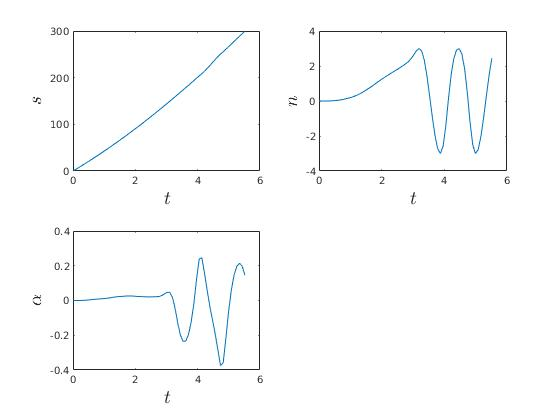
\includegraphics[scale=0.5]{hairpin_lift_curv.jpg}
  \caption{Curvilinear coordinates of vehicle in the low speed hairpin experiment.}
  \label{fig:hpcurv1}
\end{figure}
\begin{figure}[t]
  \centering
  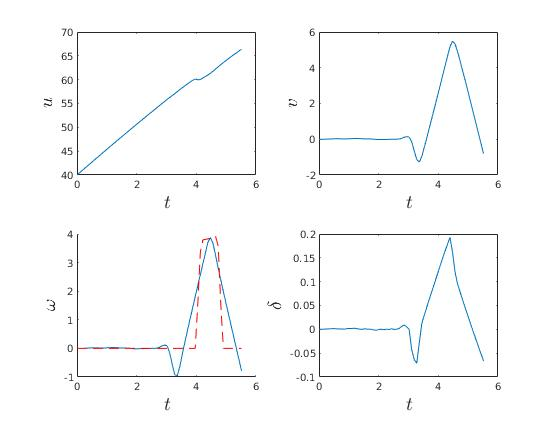
\includegraphics[scale=0.5]{hairpin_lift_cg.jpg}
  \caption{Center of gravity dynamics of the vehicle in the low speed hairpin experiment.}
  \label{fig:hpcg1}
\end{figure}
\begin{figure}[t]
  \centering
  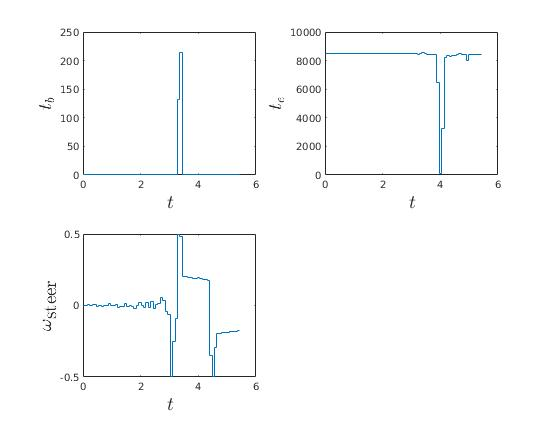
\includegraphics[scale=0.5]{hairpin_lift_u.jpg}
  \caption{Controls in the low speed hairpin experiment.}
  \label{fig:hpu1}
\end{figure}

The first sort of turn tested is the so called ``hairpin'' turn, i.e. a 180 degree turn with a small radius of curvature, in this case a radius of approximately 15 meters. Two experiments were run,
in the first the vehicle approaches the turn at a relatively slow speed of 40 meters per second and does not need to slow down to make the turn, and in the second experiment the vehicle approaches
the turn at speed of 60 meters per second and must brake in order to stay on the road and make the turn.

As shown in the resulting plots (\Cref{fig:hpcurv0,fig:hpcg0,fig:hpu0}) the controller successfully navigates a situation where it must slow down to traverse the track in a time optimal way.
The controller also takes the path through the turn with the highest radius, minimizing the need for braking and optimizing exit speed for the following straight. The low speed experiment
(\Cref{fig:hpcurv1,fig:hpcg1,fig:hpu1}) also shows an interesting behavior where the controllerstops accelerating momentarily at the highest curvature point in order to maintain tire grip.

For this scenario the no regularization method is used, and Levenberg-Marquardt constant of $0.01$.

\subsubsection{Chicane}
A further interesting experiment which was run was a squared off ``street circuit'' style chicane with two 90 degree turns, set 30 meters apart. Again the vehicle is forced to slow down to
maintain tire grip. This experiment required significant tuning and was extremely sensitive to changes in chicane length and initial vehicle velocity. For this scenario the 'convexify' regularization
method is used, along with a higher Levenberg-Marquardt constant of $0.1$.

\begin{figure}[t]
  \centering
  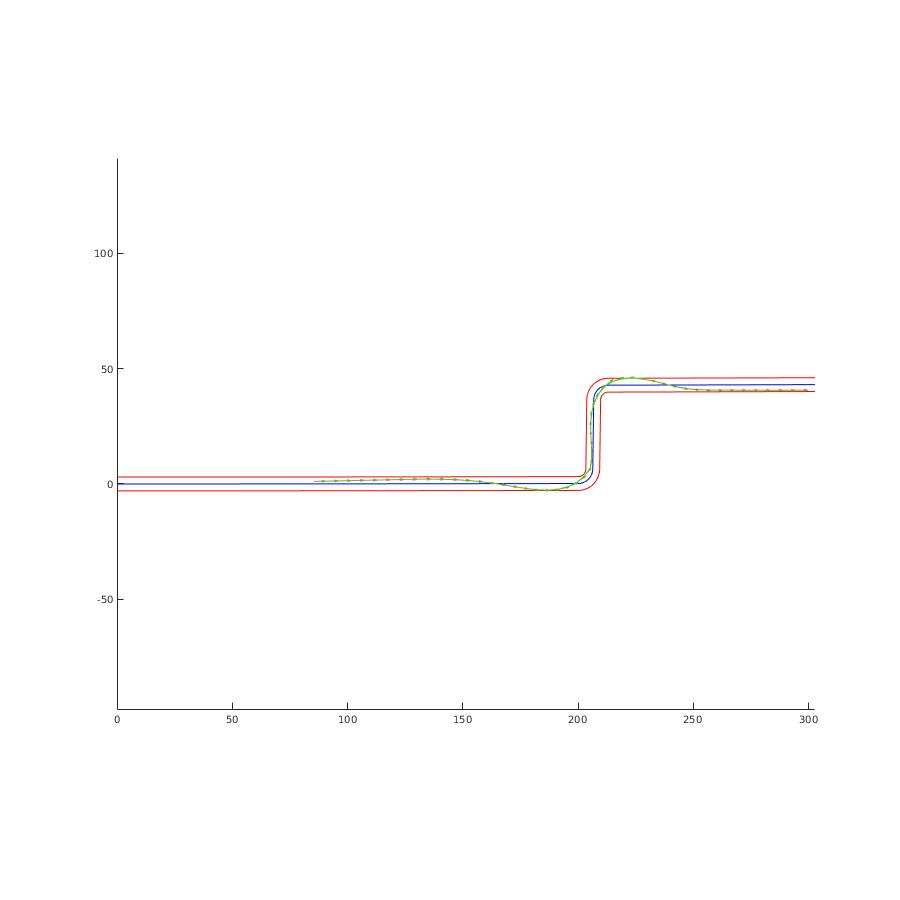
\includegraphics[scale=0.25]{chicane.jpg}
  \caption{Trajectory followed by the vehicle in the chicane experiment.}
  \label{fig:cg}
\end{figure}
\begin{figure}[b]
  \centering
  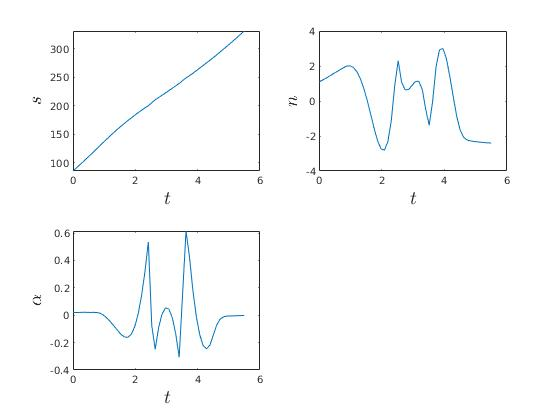
\includegraphics[scale=0.5]{chicane_curv.jpg}
  \caption{Curvilinear coordinates of vehicle in the chicane experiment.}
  \label{fig:cg}
\end{figure}
\begin{figure}[t]
  \centering
  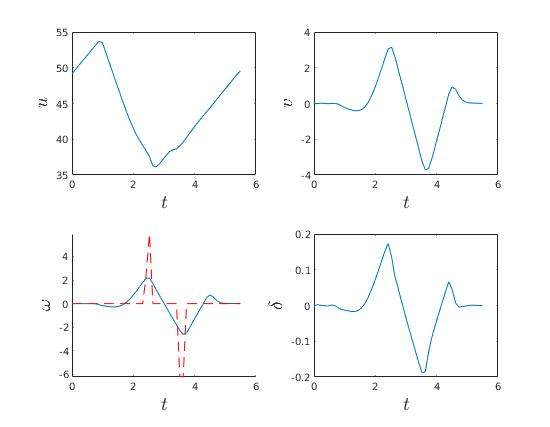
\includegraphics[scale=0.5]{chicane_cg.jpg}
  \caption{Center of gravity dynamics of the vehicle in the chicane experiment.}
  \label{fig:cg}
\end{figure}
\begin{figure}[b]
  \centering
  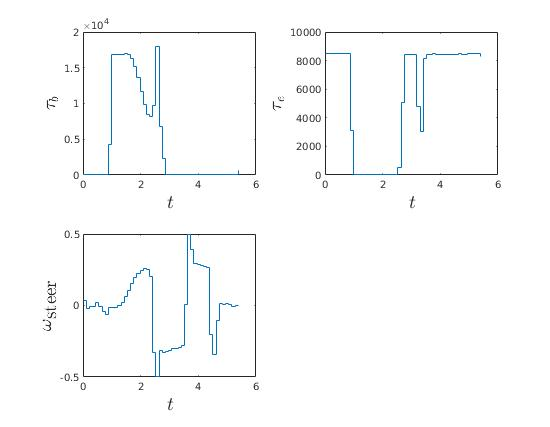
\includegraphics[scale=0.5]{chicane_u.jpg}
  \caption{Controls in the high speed hairpin experiment.}
  \label{fig:cg}
\end{figure}

It is useful to note that in all 3 of these examples the cross term for engine and brake application perform the desired purpose and prevent brake and throttle application at the same time.

Unfortunately in its current implementation, this controller runs at approximately $25$ times slower than real time when used in ordinary SQP mode. This is primarily due to the prevalence of
steps in which the solver never reaches the required tolerances, that with the 1000 maximum iterations take multiple seconds to complete. The authors could not manage to successfully get convergence
of the real time iteration even with initialization via pre solving a single SQP.

\section{Conclusions}
This project has only partially achieved it's goal of a robust time optimal model predictive controller. On one hand the formulation of the problem has successfully been proven out as viable.
On the other hand tuning requirements specific to each scenario means that the system is not sufficiently general to operate on an actual track, or when significant model-plant mismatches exist.
Once tuned the controller does however produce excellent results in difficult situations that require complex maneuvers and operates in a time optimal fashion while maintaining the physical
constraints of the vehicle. 



\section{Further Exploration}

There are several possible paths for extension to this project. The need to possibly re-formulate constraints or take advantage of other tricks to improve convergence, is a necessity.
Further exploration of nonlinear tire models would also be interesting, in particular the use of a non-smooth model instead of the oft used ``magic formula'' \cite{PAUWELUSSEN2015239}, to take
advantage of advancements in non-smooth solvers.

\bibliographystyle{IEEEtran}
\bibliography{ref.bib}
%\vspace{12pt}

\end{document}
